\part{Chiavi duplicate in alberi binari di ricerca}

\begin{tcolorbox}[colback=lightgray!20,%gray background
                  colframe=black,% black frame colour
                  arc=3mm, auto outer arc,]
                  
    \textbf{Esercizio}
    \begin{itemize}
    
    \item Vogliamo confrontare vari modi per gestire chiavi duplicate in ABR:
      \begin{itemize}
        \item implementazione "normale" (senza accorgimenti particolari)
        \item utilizzando un flag booleano
        \item mantenendo una lista di nodi con chiavi uguali
      \end{itemize} 
    \item Per fare questo dovremo:
      \begin{itemize}
        \item Scrivere i programmi Python (no notebook) che:
          \begin{itemize}
            \item implementano quanto richiesto
            \item eseguono un insieme di test che ci permettano di comprendere vantaggi e svantaggi delle diverse implementazioni
          \end{itemize}
          \item Svolgere ed analizzare opportuni esperimenti
          \item Scrivere una relazione (in LATEX) che descriva quanto fatto
          \item Nota: le strutture dati devono sempre essere implementate nel progetto; non si possono utilizzare librerie sviluppate da altri o copiare codice di altri
      \end{itemize}
    \end{itemize}
\end{tcolorbox}

\section{Spiegazione teorica del problema}

\subsection{Introduzione}
\label{sec:Introduzione_1}
In questa sezione vedremo una rapida infarinatura teorica sugli alberi binari di ricerca e sulle operazioni di inserimento e di ricerca. Per i nostri esperimenti
utilizzeremo queste due operazioni poiché il codice del inserimento lo avremo necessariamente implementato per popolare gli alberi, mentre utilizzeremo l'operazione
di ricerca poiché alla base di ogni operazione eseguibile su un ABR c'è un cammino semplice e quindi fondamentalmente una ricerca (compreso l'inserimento) e quindi i tempi di esecuzione avranno lo stesso andamento per qualsiasi operazione. 


\subsection{Aspetti fondamentali}
\label{sec:AspettiFondamentali_1}

Un albero binario di ricerca (esempio in figura \ref{fig:ABR}) è una tipologia particolare di albero binario con le seguenti caratteristiche:
\begin{enumerate}
    \item Il sottoalbero sinistro di un nodo $x$ contiene soltanto i nodi con chiavi minori della chiave del nodo $x$.
    \item Il sottoalbero destro di un nodo $x$ contiene soltanto i nodi con chiavi maggiori della chiave del nodo $x$.
    \item Il sottoalbero destro e il sottoalbero sinistro devono essere entrambi due ABR.
\end{enumerate}
Descriviamo ora le caratteristiche delle due operazioni che prenderemo in considerazione:

\begin{itemize}
  \item Per l'inserimento, iniziando dalla radice dell'albero, si sceglie ricorsivamente su quale ramo spostarsi basandoci sul confronto tra la chiave della foglia in cui
  siamo e il valore che vogliamo inserire. Arrivati in fondo all'albero creeremo un nuovo nodo, se destro o sinistro rispetto all'ultima foglia dipende 
  dall'implementazione.
  Vediamo ora la differenza tra le varie implementazioni che andremo ad analizzare, tenendo a mente che esse si differenziano solo per come gestiscono le chiavi    
  duplicate mentre hanno lo stesso comportamento negli altri casi (inserimento destro se la chiave del nuovo nodo é maggiore e sinistro se la chiave é minore).
    \begin{itemize}
      \item Classica: la chiave duplicata viene sempre inserita a destra
      \item Flag booleana: ogni nodo contiene una flag booleana che cambia il suo valore ogni volta che viene visitata da una chiave duplicata. Sinistra se la flag è True e destra se False
      \item Lista concatenta di nodi con chiavi uguali: ogni nodo viene trasformato in una lista concatenata con inserimento in testa per salvare le chiavi duplicate
    \end{itemize}
  \item Nell' operazione di ricerca per ogni foglia, prima confrontiamo il valore che stiamo cercando con quello della suddetta foglia. Se il valore è uguale allora ritorneremo
  un boolean di conferma. Se raggiunta l'ultima foglia dell'albero non trovassimo il valore allora ritorneremo un boolean di fallimento. Altrimenti se non ci
  troviamo in nessuna delle due situazioni appena descritte scendiamo l'albero con lo stesso metodo dell'inserimento. Ovviamente per fare la ricerca partiremo
  dalla radice dell'albero.
\end{itemize}

\begin{figure}[H]
  \centering
  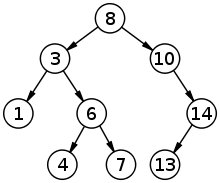
\includegraphics[width=0.35\textwidth]{Resources/ABR_Resources/ABR.png}
  \caption{Albero binario di ricerca}
  \label{fig:ABR}
\end{figure}

\subsection{Assunti ed ipotesi}
\label{sec:AssuntiEdIpotesi_1}
In un ABR le operazioni di base richiedono un tempo proporzionale all'altezza dell'albero. L'altezza attesa di un ABR costruito in modo casuale è $O(h = lg(n))$ quindi
le operazioni elementari svolte su questo tipo di albero richiedono in media $\Theta(h)$. Nel caso peggiore, il caso in cui l'albero sia completamente sbilanciato 
da un lato, dando cosi origine ad una lista, l'altezza è $\Theta(n)$ e quindi ci aspettiamo che le operazioni elementari richiedano $\Theta(n)$ per essere svolte.
Per vedere la complessità degli algoritmi più importanti di ABR basati sul caso peggiore e sul caso medio si richiama alla figura \ref{fig:ComplessitàABR} facendo
particolare attenzione ai metodi in rosso che sono quelli su cui andremo a svolgere gli esperimenti.
Poiché andremo a sperimentare su varie metodologie di inserimento è utile ipotizzare come questi avranno impatto sulle prestazioni del albero. In particolare
ci aspettiamo di vedere, in caso di un elevato numero di chiavi ripetute, una migliore prestazione nella ricerca, dovuta alla ridotta altezza del albero, utilizzando il metodo
di inserimento basato sulla lista concatenata e allo stesso modo un altezza inferiore anche per il metodo con flag booleana che dovrebbe rendere piu bilanciato l'albero 
e quindi ridurne l'altezza. 
Al contrario, il maggior numero di operazioni necessare dovrebbe rendere il metodo con lista il più lento nel inserimento di nuovi dati.

\begin{figure}[H]
    \centering
    \begin{tabular}{|c|c|c|}
        \hline
         & Complessità al caso peggiore & Complessità al caso medio\\
        \hline
        Spazio & $\Theta$($n$) & $\Theta$($n$)\\
        \hline
        \textcolor{red}{Inserimento} & $O(n)$ & $O(h)$\\
        \hline
        \textcolor{red}{Ricerca} & $O(n)$ & $O(h)$\\
        \hline
        Cancellazione & $O(n)$ & $O(h)$\\
        \hline
    \end{tabular}
    \caption{Complessità degli algoritmi di ABR}
    \label{fig:ComplessitàABR}
\end{figure}
Il nostro obiettivo in questo test è verificare sperimentalmente la veridicità delle varie complessità descritte nella figura \ref{fig:ComplessitàABR} e capire
sotto quali condizioni un albero è più conveniente di un altro, confrontandoli, a parità di numero di chiavi, in base al tempo reale che impiegano ad eseguire le operazioni.

\newpage
\section{Documentazione del codice}

\subsection{Schema del contenuto e interazione tra i moduli}
\label{sec:SchemaContenutoInterazioneModuli_1}
Per svolgere i test ho dovuto prima di tutto implementare il codice per creare la nostra struttura dati, questo avviene al interno del modulo \textbf{BST.py}. In questo modulo ho definito una classe \textbf{Tree}
il cui builder prende come input un valore che sarà la chiave della radice e la passa al costruttore della classe \textbf{Node} che crea il primo nodo del albero.
La classe \textbf{Node} definisce ogni singolo nodo del albero e il suo costruttore inizializza la variabile \textbf{key} al valore che gli è stato fornito. Questa classe, oltre agli ovvi attributi key,
left (figlio sinistro), right (figlio destro) e p (padre) contiene l'attributo \textbf{b} (boolean) per l'implementazione del inserimento con flag booleana e l'attributo \textbf{duplicate} che rappresenta
il puntatore al nodo duplicato successivo al interno della lista concatenata, in caso si utilizzi questa tecnica.
Ho successivamente creato il modulo \textbf{dataset.py} con lo scopo di generare i dati su cui eseguire i test.
In fine ho creato il modulo \textbf{benchmark.py} dove troviamo i metodi che svolgono i test.

\subsection{Descrizione dei metodi implementati}
\label{sec:DescrizioneMetodiImplementati_1}
Vediamo ora i metodi e le funzioni delle classi e dei moduli di cui finora abbiamo parlato. 

\begin{itemize}

    \item \textbf{Tree}
    \begin{itemize}
    
        \item \textbf{normalInsert(z)} : esegue l'inserimento di un nodo con chiave z con il metodo classico e restituisce a che altezza nel albero e' stato inserito il nodo.
        
        \item \textbf{booleanInsert(z)} : esegue l'inserimento di un nodo con chiave z con il metodo della flag booleana e restituisce a che altezza nel albero e' stato inserito il nodo.
        
        \item \textbf{listInsert(z)} : esegue l'inserimento di un nodo con chiave z con il metodo della lista concatenata e restituisce a che altezza nel albero e' stato inserito il nodo.
        
        \item \textbf{insert(z, insertType)} : esegue l'inserimento di un nodo con chiave z con il metodo indicato dalla variabile insertType e restituisce a che altezza nel albero e' stato inserito il nodo.
        
        \item \textbf{search(k)} : esegue la ricerca del primo nodo del albero con chiave k e restituisce a che altezza nel albero e' trovato il nodo.
                
    \end{itemize}
    
    \item \textbf{dataset.py}
    \begin{itemize}
        \item \textbf{generate\_random\_dataset(tests, times, dim)} : genera un dataset completamente casuale.
        
        \item \textbf{generate\_worst\_dataset(tests, times, dim)} : genera un dataset ordinato.
        
        \item Spiego meglio la struttura di questi dataset nella sezione \ref{sec:DatiUtilizzati_1}.
        
    \end{itemize}
    
    \item \textbf{benchmark.py}
    \begin{itemize}
    
        \item \textbf{createTree(dataset, insertionType)} : utilizzando il metodo insert della classe Tree restituisce un albero creato inserendo le chiavi contenute nel array dataset con il metodo
          indicato da insertionType.
        
        \item \textbf{benchmark(dataset, insertionType)} : la funzione crea l'albero con la funzione createTree, procede poi cronometrando il tempo di inserimento del ultimo elemento del dataset
          e infine cronometra il tempo di ricerca di un elemento scelto casualmente dal array infine calcola la media per ogni test. Le misurazioni verrano comunque spiegate più in dettaglio
          nella sezione \ref{sec:Misurazioni_1}

        \item \textbf{benchmark\_nodes(dataset, insertionType)} : la funzione ha un comportamento identico all precede pero' basando le misurazioni sul altezza del albero piuttosto che sui tempi.

    \end{itemize}
    
\end{itemize}

\newpage
\section{Descrizione degli esperimenti condotti e analisi dei risultati sperimentali}

\subsection{Dati utilizzati}
\label{sec:DatiUtilizzati_1}
Per gli esperimenti che andremo ad eseguire utilizzeremo un dataset composto da interi casuali e uno composto da interi orginati in modo da poter testare sia il caso medio che il caso peggiore. 
\begin{itemize}
  \item Random Dataset ovvero dataset di interi generati casualmente con numeri tra 0 e la dimensione del array.
  \item Worst Case Dataset ovvero un dataset ordinato in modo crescente, in modo tale da ottenere un albero completamente sbilanciato.
\end{itemize}

Ognuno di questi dataset viene generato in diverse dimensioni ( 100, 150, 200,...,4000 elementi per il caso medio e 100, 110, 120, ...,500 elementi per il caso peggiore) in modo da poter vedere
la complessità delle operazioni al crescere del dataset.
Infine ognuno di questi test viene eseguito 2000 volte per il caso medio e 200 per il caso peggiore, per poter minimizzare l'errore dovuto a fattori esterni al programma calcolando la media del tempo impiegato per ogni test.

\subsection{Misurazioni}
\label{sec:Misurazioni_1}
La funzione di benchmark riceve in input il dataset su cui deve eseguire il test e il metodo di inserimento che dovrà testare. Per ogni array nel dataset costruisce quindi un albero con il metodo di
inserimento specificato tralasciando l'ultimo elemento.
Procederà poi a cronometrare il tempo impiegato per l'inserimento del ultimo elemento simulando perciò il tempo impiegato ad inserire un dato in un albero già costruito.
In seguito cronometra la ricerca di un intero scelto casualmente al intero del array.
Questi test vengono eseguiti come detto in precedenza 2000 e 200 volte per ogni dimensione e viene calcolata una media per ogni dimensione ottenendo come output due array: un array contenente la media
dei tempi di inserimento per ogni dimensione e uno contenente la media dei tempi di ricerca per ogni dimensione. 

Per quanto riguarda la funzione di benchmark sulle altezze il funzionamento e' identico ma eseguendo misurazioni e calcoli sul altezza del albero e non sui tempi.

\subsection{Risultati sperimentali e commenti analitici}
\label{sec:RisultatiSperimentaliCommentiAnalitici_1}

\subsubsection{Inserimento}

\begin{figure}[H]
  \centering
  \begin{minipage}{.5\textwidth}
    \centering
    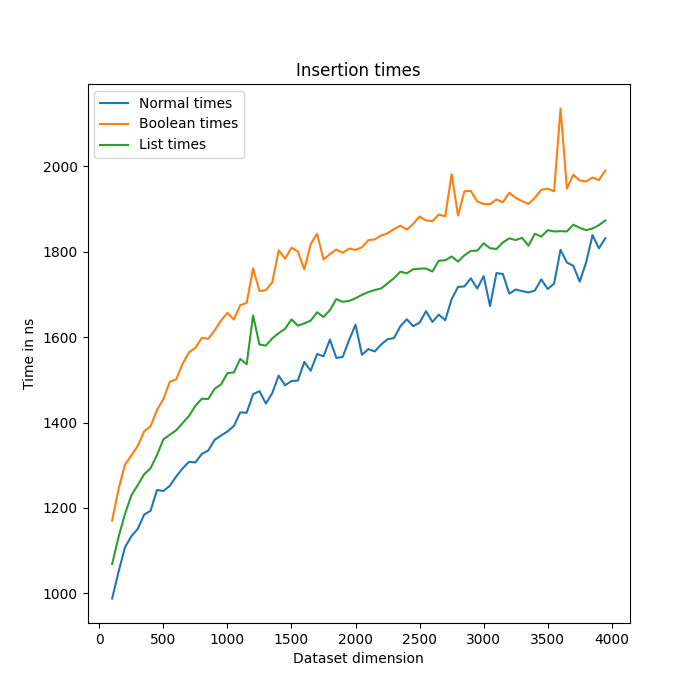
\includegraphics[width=0.7\linewidth]{Resources/ABR_Resources/InsertionTimes.png}
    \caption{Tempi di inserimento}
    \label{fig:InsTimes}
  \end{minipage}%
  \hfil % Add space between minipages
  \begin{minipage}{.5\textwidth}
    \centering
    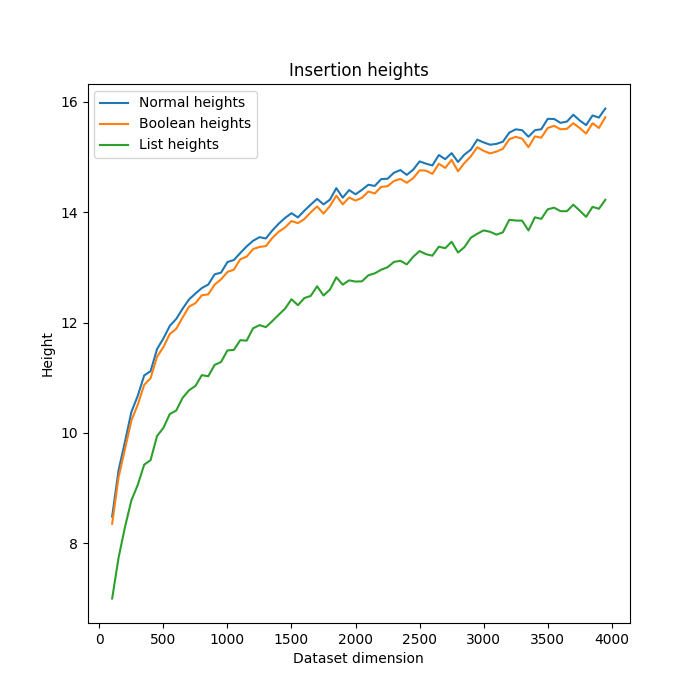
\includegraphics[width=0.7\linewidth]{Resources/ABR_Resources/InsertionHeights.png}
    \caption{Altezze per inserimento}
    \label{fig:InsHeights}
  \end{minipage}%
\end{figure}

Iniziamo subito notando come i risultati del test che vediamo in figura \ref{fig:InsTimes} confermino quanto ipotizzato dalla nostra analisi teorica nella sezione \ref{sec:AssuntiEdIpotesi_1},
ottenendo $\Theta(h)$ come andamento delle operazioni di inserimento sui dataset che rappresentano il caso medio.
Andando più in dettaglio con l'analisi possiamo notare come l'algoritmo classico risulti il più rapido, seguito poi dalla lista concatenata e infine dalla flag booleana. 
A differenza di quanto ipotizzabile, data la maggiore complessità delle operazioni per la creazione della lista concatenata, l'algoritmo con lista risulta più prestante di quello booleano probabilmente
aiutato dal fatto che incorporando i nodi uguali in uno solo riduce l'altezza del albero e quindi il numero di cicli necessari per l'inserimento, come evidenziato in figura \ref{fig:InsHeights},
a differenza della flag booleana che si limita a cercare di bilanciare meglio l'albero, mantenendo però il numero di nodi invariato.

\begin{figure}[H]
  \centering
  \begin{minipage}{.5\textwidth}
    \centering
    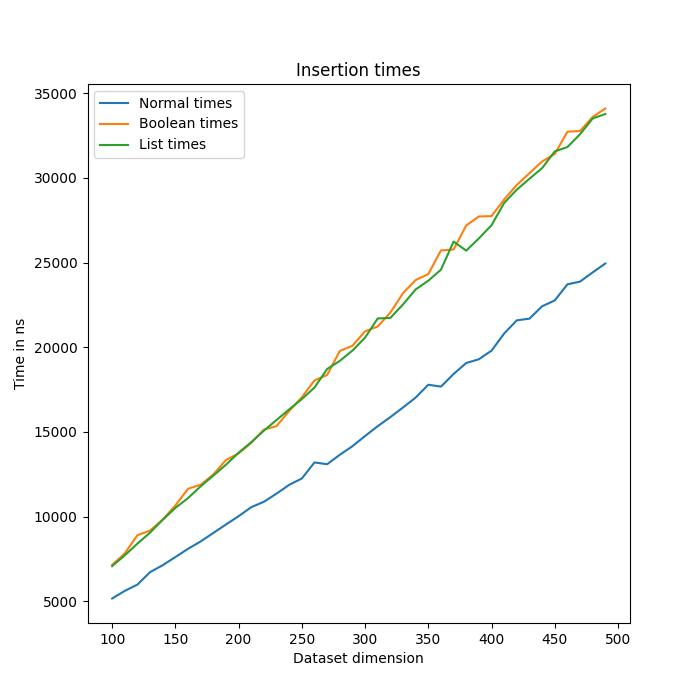
\includegraphics[width=0.7\textwidth]{Resources/ABR_Resources/WorstInsertionTimes.png}
    \caption{Tempi di inserimento caso peggiore}
    \label{fig:WInsTimes}
  \end{minipage}%
  \hfil % Add space between minipages
  \begin{minipage}{.5\textwidth}
    \centering
    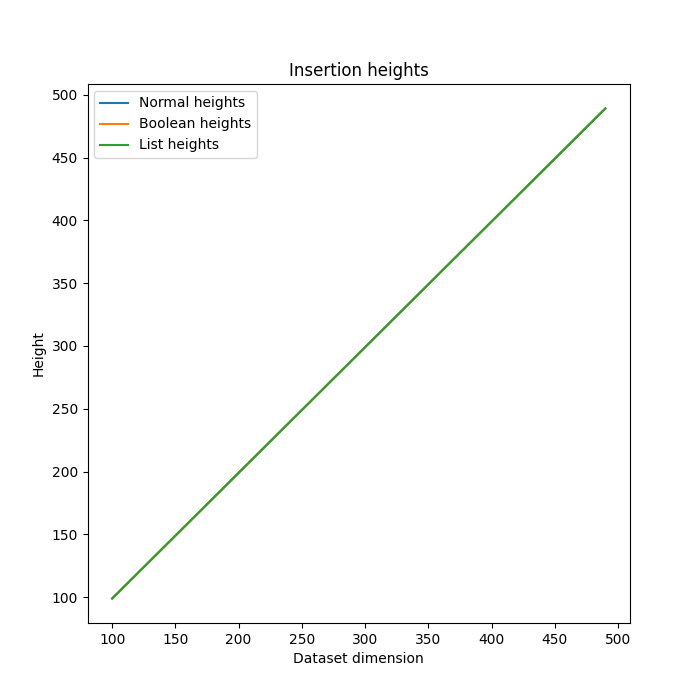
\includegraphics[width=0.7\textwidth]{Resources/ABR_Resources/WorstInsertionHeights.png}
    \caption{Altezze per inserimento caso peggiore}
    \label{fig:WInsHeights}
  \end{minipage}%
\end{figure}

Anche per quanto riguarda i risultati mostrati in figura \ref{fig:WInsTimes} possiamo notare come gli esperimenti abbiano confermato la nostra analisi teorica mostrando un andamento $\Theta(n)$ per tutti
gli algoritmi nel caso peggiore. Non ci sorprende vedere come l'algoritmo classico risulti il più rapido, in quanto per tutti e tre gli algoritmi viene creata una lista nel caso peggiore e l'algoritmo
classico e' quello che utilizza meno operazioni per farlo, permettendo cosi di ottenere i risultati migliori.
Possiamo notare invece che gli altri due algoritmi hanno prestazioni pressoche' identiche.

\subsubsection{Ricerca}

\begin{figure}[H]
  \centering
  \begin{minipage}{.5\textwidth}
    \centering
    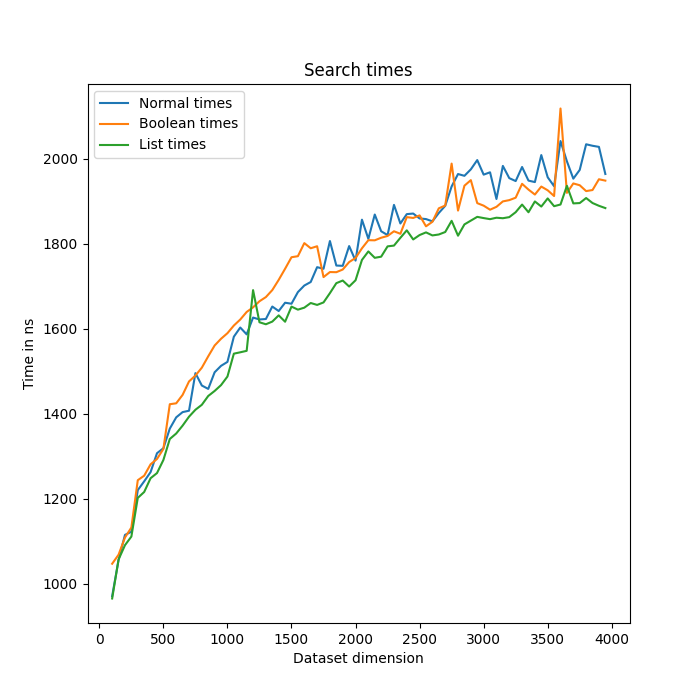
\includegraphics[width=0.7\textwidth]{Resources/ABR_Resources/SearchTimes.png}
    \caption{Tempi di ricerca caso medio}
    \label{fig:STimes}
  \end{minipage}%
  \hfil % Add space between minipages
  \begin{minipage}{.5\textwidth}
    \centering
    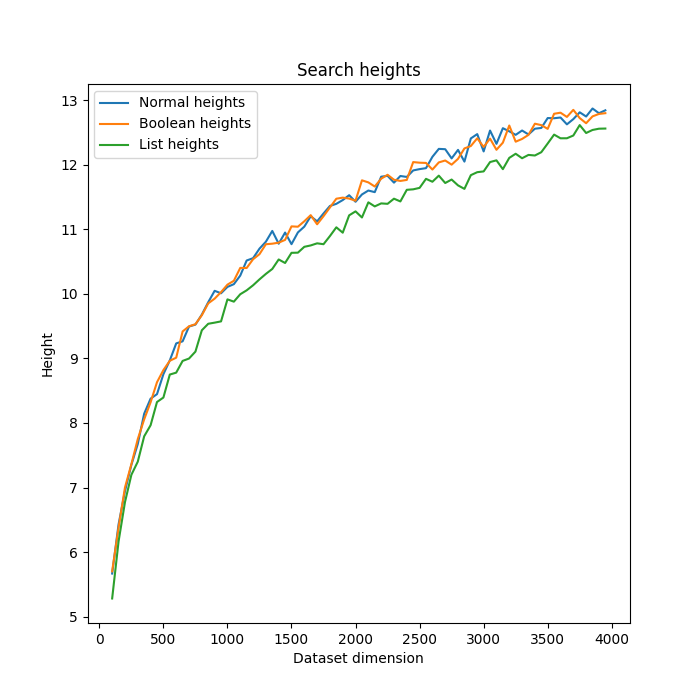
\includegraphics[width=0.7\textwidth]{Resources/ABR_Resources/SearchHeights.png}
    \caption{Altezza per ricerca caso medio}
    \label{fig:SHeights}
  \end{minipage}%
\end{figure}

Per quanto riguarda le prestazioni della ricerca mostrate in figura \ref{fig:STimes} possiamo notare come i risultati sperimentali abbiano confermato le nostre
ipotesi con un andamento $\Theta(h)$.
Salta subito al occhio come le prestazioni siano quasi identiche per tutti gli algoritmi con un leggero miglioramento per quanto riguarda l'algoritmo a lista concatenata.

\begin{figure}[H]
  \centering
  \begin{minipage}{.5\textwidth}
    \centering
    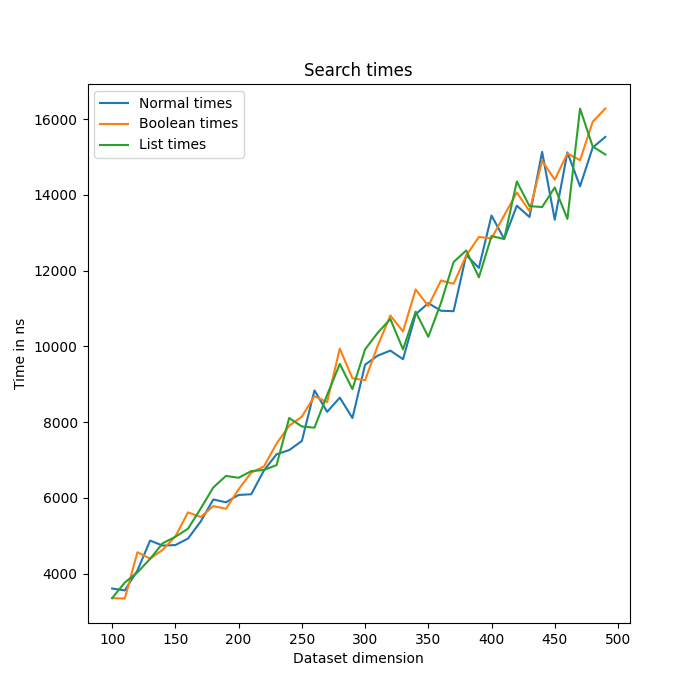
\includegraphics[width=0.7\textwidth]{Resources/ABR_Resources/WorstSearchTimes.png}
    \caption{Tempi di ricerca nel caso peggiore}
    \label{fig:WSTimes}
  \end{minipage}%
  \hfil % Add space between minipages
  \begin{minipage}{.5\textwidth}
    \centering
    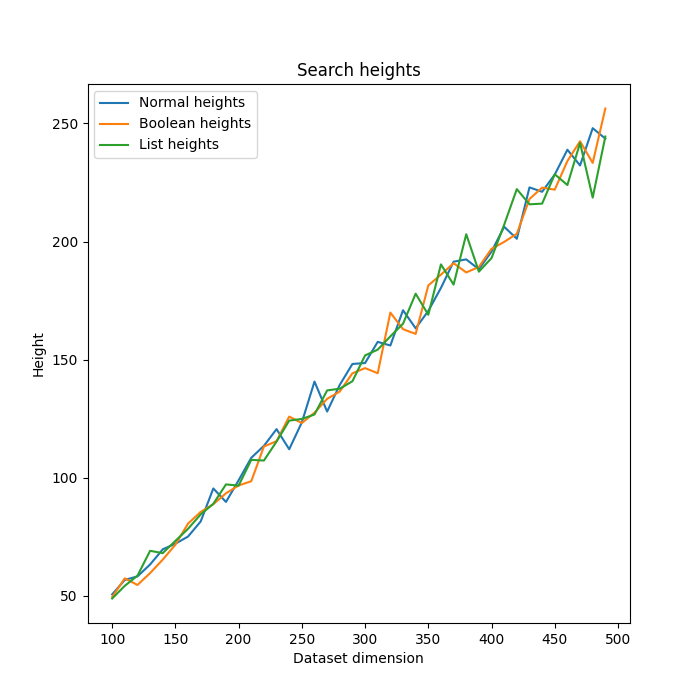
\includegraphics[width=0.7\textwidth]{Resources/ABR_Resources/WorstSearchHeights.png}
    \caption{Altezza per la ricerca nel caso peggiore}
    \label{fig:WSHeights}
  \end{minipage}%
\end{figure}

Come per i casi precedenti anche nel caso peggiore i risultati in figura \ref{fig:WSTimes} sono concordanti con la nostra previsione di una complessità $\Theta(n)$.
In questo caso gli algoritmi sembrano avere prestazioni quasi identiche, non identificando cosi' un algoritmo preferibile per questa situazione.


\subsection{Tesi e sintesi finale}
\label{TesiSintesiFinale_1}
Riassumiamo adesso cosa possiamo estrapolare dai nostri test:
\begin{itemize}
    \item Entrambi i metodi analizzati hanno complessità $\Theta(h)$ nel caso medio come avevamo previsto nell'analisi teorica.
    \item I due metodi nel caso peggiore hanno complessità $\Theta(n)$ confermando l'analisi teorica.
    \item Il metodo classico risulta essere il piu prestante sia nel caso medio che nel caso peggiore per quanto riguarda l'inserimento seguito dal metodo con lista e infine quello booleano.
    \item Nella ricerca il metodo con lista concatenata riuslta essere il piu prestante seguito dai metodi classico e con flag booleana anche se nessuno dei tre spicca particolarmente rispetto agli altri.
    \item Nella ricerca tutti i metodi risultan equivalenti nel caso peggiore.
\end{itemize}



